\documentclass{report}
\usepackage{graphicx}
\usepackage{assymb}

\usepackage[utf8]{inputenc}
\usepackage{hyperref}
\hypersetup{
    colorlinks=true,
    linkcolor=blue,
    filecolor=magenta,      
    urlcolor=cyan,
    pdftitle={Overleaf Example},
    pdfpagemode=FullScreen,
    }
    
\title{Lully: a crowdsource approach to argument corpus generation DRAFT}
\author{Stanislaw Malinowski
\\[1cm]{\small Advisor: Rob Gaizauskas}
\\[1cm]{\small Module Code: COM3610}
}

\urlstyle{same}
\date{\today}

\usepackage{array}

\newenvironment{conditions}
  {\par\vspace{\abovedisplayskip}\noindent\begin{tabular}{>{$}l<{$} @{${}={}$} l}}
  {\end{tabular}\par\vspace{\belowdisplayskip}}

\usepackage{biblatex}
\addbibresource{Dissertation.bib}

\usepackage{booktabs}
\usepackage{enumitem}

\linespread{1.25}

\begin{document}
\maketitle
\section*{Title page}
This report is submitted in partial fulfillment of the requirement for the degree of BSc in Computer Science by Stanislaw Malinowski.
\newpage

\section*{Declaration}
All sentences or passage quoted in this report from other people's work have been specifically acknowledged by clear cross-referencing to author, work and page(s). Any illustrations that are not the work of the author of this report have been used with the explicit permission of the originator and are specifically acknowledged. I understand that failure to do this amounts to plagiarism and will be considered grounds for failure in this project and the degree examination as a whole.

Stanislaw Malinowski
\newpage

\section*{Abstract}

Lully project is a gamified crowdsource data capture tool with the goal of creating argument databases. Gamification follows the Game With A Purpose paradigm pioneered by von Ahn, and present in applications such as Google Crowdsource and Duolingo. The created argument database could be used to create machine learning models that can extract argument structure from raw text.
The achieved status of the project is a proof-of-concept with 6 games that create the corpus and a rudimentary gamification layer. That falls short from the original project outline that assumed deployment and testing the application with real users, and creating a corpus of structured arguments. 

\newpage

\section*{Acknowledgements}
I would like to thank my supervisor, Rob, for his patience and guidance, and Jonathan, a PhD student, for reviewing my work. Their feedback and support have been invaluable to my academic progress.

\newpage

\tableofcontents

\newpage

\chapter{Introduction}
How to make a machine understand argument structure?
That is a very relevant question. Arugment mining does not have as much interest as other NLP (Natural Language Processing) areas, such as sentiment analysis, with market \href{https://www.polarismarketresearch.com/industry-analysis/sentiment-analytics-market}{valued} at \$3.15 billion in 2021.

The base resource for any NLP task is the dataset, its quality and size impactful on any subsequent processing. Argument mining does not have enough open access datasets with high quality structured argument data.  Expert annotation is high quality but costly, and crowdsourcing suffers from low quality. 

The goal of this project is to explore the possiblities for a tool that solve this tradeoff and deliver high-volume, high-quality data at a low cost. 
The main concept behind this is the use of Games with A Purpose Paradigm to drive user engagement as opposed to using paid workers. User acquisition, retention and engagement is managed through various incentives. 

The resulting corpus could be used by NLP researchers as a labeled dataset. NLP programs trained with it should be able to comprehend and create debate-like discourses across domains.

This project is an exploratory one, aiming to create a design and functionalities list, rather than a full-fledged product.
Design is provided and some of the functionalities were done as a proof-of-concept. 
That is on the spectrum of design -> proof of concept -> prototype -> MVP (Minimum Viable Product).

Functionalities include but are not limited to: users viewing a constructed argument tree and interacting with it to expand it, import of data from existing argument schema projects, a variety of minigames that compose the corpus. 

This report will go over the relevant literature, including human annotation schemas, and semi-supervised learning approaches, then review similar software. That is used to create a list of capabilities to explore, grouped by priority. Based on that a broad-scope design is created, and implementation presented of the highest priority aspects of the project.
That section will be the basis for development of a more technical design document on a later date.
Report will end with a description of achievements to date and plans for the future.

\section{Guding example}

Let us take a topic frequently mentioned in current debates: Universal basic income should be implemented.
Various iterations of the arguments for this statement and associated data structures will accompany many sections of this paper.

\newpage

\chapter{Literature Survey}
Argument structure analysis goes back to antiquity. \cite{angelelli_techniques_1970}
Analysis of argumentation has been an active topic in numerous research areas, such as philosophy \cite{van_eemeren_systematic_2003}, communication studies \cite{mercier_why_2011}, and informal logic \cite{blair_informal_2000}, among others. This chapter will cover the areas that this project touches. There are several types of approaches. Fully annotated and semi-supervised approaches.

\href{https://en.wikipedia.org/wiki/Semantic_network}{Semantic network} are graphical representations of concepts and their interrelationships, often used in natural language processing and artificial intelligence. It is closely related to 'formal concept analysis', which is an activity in philosophy aiming at a similar results. Finally ontology languages are the static, completed equivalent. They are often created synthetically, as opposed to the analytic origin of the previous ones.

\section{Background}
From Stoic Logic to Leibniz's Characteristica Universalis, there were attempts to understand, map and summarize arguments expressed in common language. 
\cite{woltzenlogel_paleo_leibnizs_2016}
*Elements of Logic*, a logic textbook from 1826 by Richard Whatley introduced the modern arrow based logic notation. It was elaborated in 1913 by John Henry Wigmore.
\cite{wigmore_principles_1913}

\href{https://commons.wikimedia.org/wiki/File:Whatley.png}{Whatley's notations image}

Second half of the 20c saw a computerized analysis become a reality. Bag of word approaches have been seen \href{https://www.tandfonline.com/doi/abs/10.1080/00437956.1954.11659520}{as early as 1954}...
\cite{harris_distributional_1954}

Logic programming languages were the next step, with \href{https://en.wikipedia.org/wiki/Planner_(programming_language)}{Planner} as the pioneer in the field, even if not exactly with *personal* applications in mind.  It was created in 1969 with the main feature being forward and backward chaining of statements to prove a given goal statement.
\cite{hewitt_planner_1970}

Its function was *synthetic*, not analytic - so the reverse of argument mining. Nevertheless, it is an interesting reference point.

Jumping forward, after AI winters Machine Learning revolution of the 2010s going into 2020s has been fueled by data created by the previous decades of the internet. Image diffusion models such as Stable Diffusion are using existing works of art, a legally controversial issue. LLMs such as GPT series use Wikipedia and \href{https://paperswithcode.com/dataset/webtext}{WebText} dataset.
\cite{rombach_high-resolution_2022}

Argument mining is lagging behind the trailblazing subdisciplines of machine learning. The problem in many studies of argumentation is the undersupply of data. Yet there is plenty of online discourse.
There is abundance of linear, monologue data but adversarial labeled data is scarce. That is an obstacle to development of adversarial NLP models that could be used in chatbots. 

Online platforms, such as reddit, quora, twitter are host to the most resounding debates, heard by hundreds of millions.  Discussions topics include current political controversies, religious questions and lore discussions. These discussions form the core of the public discourse in modern society.  The results are limited, as opinions gathered in this way are devoid of explicit reasoning structure.  The act of commenting online corresponds to 'claiming ownership for a new piece of knowledge' \cite{teufel_scientific_2014} Expressing arguments for, negotiating compromises, pursuing social shifts, finding or failing-to-find common ground - are all different types of discourses. The usual output is a series of posts, comments or tweets, that are under structured. 
Previous studies included attempts to automatically derive representations of the discourse structure from unstructrued text \cite{abbott_how_2011}
The main drawback is the annotation cost, using dozens of hours of expert work, and tens of pages of annotation manuals.

Notable projects in the area include IBM's \href{https://research.ibm.com/interactive/project-debater/}{Project Debater} \cite{slonim2021autonomous}, yet these are not open sourced.

\section{Comparison to previous papers}
The results obtained in this project, the proof of concept for crowdourced sourcing of argument mining labeled data, play into the previous papers in the argument mining field.
Lully avoids the multi-page annotation pitfall of other studies \cite{teufel_towards_2009}.
The main intellectual debt is to von Ahn 2008 'Games with a purpose, as well as \href{https://dl.acm.org/doi/10.1145/2448116.2448119}{Phrase detectives}.
\cite{poesio_phrase_2013}

When taking features of Lully that aggregate input of multiple users, (Wyner et al 2015 - arugment discovery and extraction with the Argument Workbench) seems quite similar. Argument Workbench also focuses on textual data, not adversarial one. 

In fact the PostgresSQL schema arrived at is quite similar to the one by 
\cite{abbott_internet_2016}

An approach directly competing with the one Lully takes is by Wachsmuth et al 2017 'building an argument search engine for the Web' that scrapes existing data sand serves it through a ssearch engine.
\cite{wachsmuth_building_2017}

\cite{fromm_towards_2022}

Another recent approach to the issue is the TARGER project, a native PyTorch embedding that uses neural networks for argument mining

\cite{chernodub_targer_2019}

\section{Annotation}
There are different strategies for annotation. Much of the study of argument annotation has focused on citation function in scientific papers.
Many annotation schemas for argument citation motivation have been created \cite{teufel_scientific_2014}, \cite{mann_rhetorical_1987} and had success in research.
These studies work by outlining analytically from a sample of essays, articles or other texts, an exhaustive list of types of roles of statements.
Then the researchers proceed to create a long, multi-page annotation guidelines. Up to 111 sides of A4 in some cases! \cite{teufel_towards_2009}
As the next step, annotators are selected. Some studies choose discipline experts, some on purpose select persons not familiar with the discipline.
That is done in order to increase domain-independence of the annotation schema.
The following step is usually to collate the annotations created by the annotators. 

There is existent discussion \cite{artstein_inter-coder_2008} of various algorithms for this purpose.

In summary, the pure annotation strategy is costly but its experiences are quite helpful. The basic information flow pipeline is shown in (Razuvayevskaya and Teufel 2017 - finding enthymemes in real-world text - a feasibility study) as a 5 part process.
\begin{quote}
   mining: argument extraction, segmentation, i.e. identification of minimal argumentative discourse units (ADUs), segment classification, i.e. labeling of ADUs based on their argumentative roles, identification of relations between these segments, and argument completion, i.e. automatic construction of statements from implicit propositions
\end{quote}
\cite[page 114]{Tefuel2017}


The latter part includes enthymeme decection, which is defined as:
\begin{quote}
According to the Aristotelian definition [6], enthymemes are standard-form syllogisms with one missing proposition.  (ibid.)
\end{quote}
\cite[page 113]{Tefuel2017}

\section{Annotation with crowdsourcing}
A number of researchers have explored the crowdsourcing area of the potential solution space to the problem of argument structure extraction.
Following (von Ahn, 2008), we can distinguish between 3 types of approches to crowdsourcing with respect to the type of incentive provided to the participants.
There is the financial approach, the altruistic approach, and the gamification (enjoyment) approach. Papers reviewed did not feature the enjoyment approach.

Starting chronologically, the first paper is Anand et al 2011 "How can you say such things?!?: Recognizing Disagreement in Informal Political Argument".
One of the features of this paper to note is its use of Amazon's "Mechanical Turk" service for contributions. Paid volunteers ('Turkers') did the annotations. 
Corpus derived from a form '4formums.com' and focused on US dicourse on topics such as: evolution, gun contorl, abortion and gay marriage. A collection of posts and comments was used to define QR (quote-response) pairs where one user's text Q was quoted by another one, with some added commentary R. The Turkers had a [-5, 5] scale to indicate agreement or disagreement in the pair.

Other dimenions of the QR relationship were explored beyond 'agree/disagree': 'fact/emotion/, 'attack/insult', 'sarcasm', 'nice/nasty'

That was compared to expert performance, using Krippendorff's 'alpha' indicator.

Another example comes from (Wyner et al 2015 ).

Quotes are a description of the tool
\begin{quote}
 ArgumentWorkbench, which is a interactive, integrated, modular tool set to extract, reconstruct, and visualise arguments. [...]
\end{quote}
\begin{quote}
 The Argument Workbench is a processing cascade, developed in collaboration with DebateGraph. [...]
\end{quote}
\begin{quote}
 it is an open source desktop application written in Java that provides a user interface for professional linguists and text engineers to bring together a wide variety of natural language processing tools and apply them to a set of documents
\end{quote}

It is worth noticing that they used a desktop application. The other option being mobile application. There are tradeoffs visible.
Mobile applications do not have the 'screen real estate' for complex interfaces, yet higher number of people use them. Over \href{https://gs.statcounter.com/platform-market-share/desktop-mobile-tablet}{50\% more people use mobile}.

For low-entry-cost crowdsourcing approach that is essential.
Then the authors mention the workflow, and attach a diagram.
\begin{quote}
 We harvest and preprocess comments; highlight argument indicators, speech act and epistemic terminology; model topics; and identify domain terminology.
\end{quote}
\begin{quote}
 we use the GATE framework (Cunningham et al.(2002)) for the production of semantic metadata in the form of annotations
\end{quote}

\section{Extant corpora}
There are some ready corpora for argumnet mining.

Studies mention source data themselves. 
For instance, (Awadallah, Ramanath, and Weikum 2012 Harmony and dissonance: organizing the people's voices on political controversies)
say the following:
\begin{quote}
 For matching names in text sources against canonical entities, we leverage existing knowledge bases like DBpedia, Freebase, or Yago.
\end{quote}

Moreover, \href{https://direct.mit.edu/coli/article/45/4/765/93362/Argument-Mining-A-Survey}{Argument mining survey} mentions many of them.
\begin{quote}
 Internet Argument Corpus (IAC) (Walker et al. 2012) is a corpus for research in political debate on Internet forums. It consists of approximately 11,000 discussions, 390,000 posts, and some 73,000,000 words
\end{quote}
\begin{quote}
 AIFdb17 (Lawrence et al. 2012), containing over 14,000 Argument Interchange Format (AIF) argument maps, with over 1.6m words and 160,000 claims in 14 different languages.18 These numbers are growing rapidly, thanks to both the increase in analysis tools interacting directly with AIFdb and the ability to import analyses produced with the Rationale and Carneades tools (Bex et al. 2012). Indeed, AIFdb aims to provide researchers with a facility to store large quantities of argument data in a uniform way. AIFdb Web services allow data to be imported and exported in a range of formats to encourage re-use and collaboration between researchers independent of the specific tools and data format that they require.
\end{quote}
\href{https://corpora.aifdb.org/}{Link to AIFdb}.

Both corpora focus on manual labeling.
The Argument Interchange Format is a valid standard for any argument crowdsourcing project to follow.  This standardized JSON graph format make data transport and display easier. That is a great opportunity as their platform features a display tool.  The project can leverage this external tool and standard and focus on other features of the crowdsourcing process.
Another resource of arguments online is the `args.me` online resource. 
Its creation was described in Wachsmuth et al 2017

Args.me has an exposed search API and database schemas. The paper also emphasises the ethical choice contained in the construction of personalized search.
It also mentions the high cost of the long hours of expert time.
Another resource is the \href{http://araucaria.computing.dundee.ac.uk/}{Araucaria} program, mentioned by several papers. Link provided seems to be broken, though. 

There are cons to the current corpora, though.
Only few publicly available argumentation corpora exist, as annotations are costly, error-prone, and require skilled human annotators (Stab and Gurevych, 2014a; Habernal et al., 2014).
Although argumentation mining in user-generated Web discourse has a long way to go (my  methods currently achieve only about 50\% of human performance)

\section{Mixed approaches}
The above approaches were deemed to be limited. In fact, there seems to have been a shift in approaches around 2014.
There has been an argument that automatic processing is preffered due to the cost, unreliablity of annotations and scarcity of trained personnel
(Stab and Gurevych, 2014a; Habernal et al., 2014)
With that being the turining point, the efforts thereafter have focused on putting the main weight of the process on automatized process. 
That reflects the wider industry shift towards the use of Machine Learning over the past 10 years.

Researchers conceded that manual analysis is not feasuble some studies (Habernal and Gurevych 2015 - exploiting debate portals for semi-supervised).
They attempted to bypass that problem using semi-supervised learning.

Another approach is a blending approach. That consists in adding small amount of high quality and manually labeled data.
That vein of thought is explored in (Will it Blend? Blending Weak and Strong Labeled Data in a Neural Network for Argumentation Mining Eyal Shnarch et al.
ACL, 2018 http://aclweb.org/anthology/P18-2095)
Existence of this approach fares well for the crowdsourcing approach. Primarily the data will be strongly labeled, but if it proves weak for training using ML techniques, 
supplementation with weakly labeled data will be saving the utility of crowdsourced data.

Another attempt was this paper (Al-Khatib et al 2016 - crossdomain mining of argumentative text through Distant Supervision).
This study makes the strongest case for the exclusion of crowdsourcing as a means of data acquisition.
\begin{quote}
 Studies reveal that annotators need multiple training sessions to identify and classify argumentative segments with moderate inter-annotator agreement, and crowdsourcing-based annotation does not help notably (Habernal et al., 2014)
\end{quote}
Of note is also the source of the data. Authors say
\begin{quote}
 we acquire a large corpus with 28,689 argumentative text segments from the online debate portal idebate.org. The corpus covers 14 separate domains with strongly varying feature distributions.
\end{quote}
This source is highly specifc. That argumentative discourse is not a representative sample of human argument space. Verbal arguments
also experts 

These arguments are put into the search system using the PageRank algorithm \cite{brin_anatomy_1998}.  That gives grounds to considering that algorithm a good basis for a ranking of arugments in other circumstances.

\section{Games with purpose to the rescue}
A guiding paper to this area of literature review was \cite{von_ahn_designing_2008} 
In the 'games with purpose' paradigm, we expect users to contribute for their own enjoyment. Enjoyment maximization should result in a higher number of Average Lifetime Contribution.  A spotless user flow and an intuivie application are of the highest priority to achieve that.

How to apply this approach? The paper describes what makes games successful.
These are three main factors: enjoyment, timed response, ELO system.
"Enjoyment" is not defined formally there, but simply a result of knowing the games by their fruits:

\begin{quote}
 The key property of games is that people want to play them. We therefore sidestep any philosophical discussions about “fun” and “enjoyable,” defining a game as “successful” if enough human-hours are spent playing it
\end{quote}
That  *a posteriori* feature can be predicted by keeping the right level of challenge in front of the player.  \cite{locke_theory_1991}
Right level of challenge is measured through a 'timed response' mechanic built into the game.
The player's skill is evaulated on the basis of duration of the task. 
Self awareness of the speed of execution and the increasingly narrowing bar representing time left provides live feedback.
\href{https://en.wikipedia.org/wiki/Elo_rating_system}{ELO system} ensures that in player versus player games there is balance. Each player can't go against player very far from their own skill level.
Moreover, it exploits the competitive desire in humans.
The social factor seems valued in games as competitive sports are a growing market, with nearly 2 million US dollars revenue \href{https://www.statista.com/statistics/490522/global-esports-market-revenue/}{predicted} in 2025

Social factors have not been observed to feature in the studies mentioned so far.
There was no competitiveness, the workflow was each annotator working individually.
There was no incentive for agreement between annotators.
This is a limnitation that could be overcome.

The other takewaway is a set of metrics. These are
- labels per human hour
- Average Lifetime Play
While the first one is self-explanatory, the second might not be.
Study describes the latter as 
\begin{quote}
 ALP is the overall amount of time the game is played by each player averaged across all people who have played it. For instance, on average, each player of the ESP Game plays for a total of 91 minutes.
\end{quote}
Average score of 91 minutes is a good benchmark to compare with.

Phrase detectives \cite{poesio_phrase_2013} is the leading example of the use of the 'game with purpose' paradigm in order to gather data for NLP research.
ALP of only 30 minutes. It seems there is a a headspeace to improve on that. nothing indicates that this area has hit a ceiling.
What they excel at is: 'task completion, scoring and storyline as a seamless experience'
These are qualities worth emulating. Task completion and scoring are the easiest to implement. 
In contrast, creating a coherent and engaging storyline would require a specific skillset that might not always be available.
Possibly emphasizing social features could substitute this.

% todo similar game, only web
tileattack game
https://tileattack.com/?ref=ldc

\section{Similar software review}
There is a plethora of similar software. These can be found in many types, differing by platform and target audience. Many of those are outdated.
The similar software can be dividd intothe following types:
- commercial B2B SAAS solutions
- hacker-ethics personal knowledge management tools.
- is also a record of software developed specifically for research.

\subsection{Business solutions}
Commercial solutions aim to help in meetings, by providing a way to write structured notes and diagrams. These often have a rich user interface, focusing on graphics and interactivity.
Data portability and breadth of access are less of a concern in that case.
There are many companies offering business-to-business services in NLP.  These range from meeting minutes or report summaries, live structured note taking, visualization software, or customer sentiment analysis.  Business model is frequently 'freemium', where users can use the app for free, but some features are hidden behind a paywall.

\href{https://lexikat.com/#/}{Lexikat} provides "no-code concept maps and text analysis models from any document." It is a Natural Language Processing platform that companies pay for access to in order to analyze data and create reports. There is not much that can be applied to the Lully project from this technology.

On the other hand, \href{https://infranodus.com/}{Infranodus} is a multi-purpose analytics tool for extracting arguments and enhancing them through various AI techniques. Their main selling point is visualization capabilities and network representation of knowledge. That holistic approach is definitely useful in many contexts, yet the argument structure for argument mining seems more tree-like in most cases.

\href{https://www.mindmup.com/}{Mindup} is a browser based tool for creating mind maps for individuals and organizations. It was to be open source until 2017 with limited use clause, but since then has gone to a freemium model and closed source. They provide a website and a chrome extension. The web version provided is theoretically dedicated to argument struture, yet in practice similar results could be achieved with other free software, such as \href{https://www.canva.com/}{Canva}. One can create an argument representation and save it as an image, possibly share it with other users, but that is all.

\href{https://en.wikipedia.org/wiki/Crowdsource_(app)}{Google Crowdsource} is a tool created by Google to create datasets for their ML team. The app features multiple tasks of varying difficulty, focusing mainly on image labeling, but also audio recognition. What is the most relevant in this project in the context of Lully is the reward scheme, or gamification. It is quite simple indeed, especially compared to many purely games. The whole mechanism has two parts: stats and badges. Stats are for number of contributions and their accuracy. There is little use in data from a user that does creates many labels that aren't validated by others as correct. Badges provide more of the granular feedback, encouraging the user to explore different areas of the application. These features are quite easy to transplant.

\section{Reply protocols}
That type of games was examined in Prakken 2005. Distinguished different types of 'reply protocols':
\begin{quotation}
  Dialogue systems can vary in their structural properties
in several ways: whether players can reply just once to the other player’s moves or may try
alternative replies (unique vs. multi-reply protocols); whether players can make just one or may
make several moves before the turn shifts (unique vs. multi-move protocols); and whether the turn
shifts as soon as the player-to-move has made himself the winning side or may shift later (immediate
vs. non-immediate-reply protocols)
\end{quotation}
\cite[page 1010]{prakken_coherence_2005}

The configuration space is non-trivial, and the choice which of these protocols would be implemented in the game needs to be pondered.
Playtesting is needed to make sure these assumptions work out, maybe 2 or 3 move points per player (new node allowance) would be better.
These can be conceputalized as restrictions compared to a 'multi-reply, multi-move, non-immediate-reply' variant.

Let us illustrate this with an example using the above UBI statement. Imagine two players, Alice and Bob in a game.
Alice supports the statement ("Universal basic income should be implemented."). And presented an argument for it, A:
UBI can reduce poverty and inequality.

She has one more argument to support it in mind, B.
UBI can promote entrepreneurship and innovation by allowing individuals to take risks without the fear of financial insecurity.

Bob has in mind the following arguments against the root statement, let us call this set X:
- UBI can lead to inflation and decrease the value of currency, causing more harm than good. //
- UBI can discourage people from working and contribute to a decline in productivity, which can have  negative effects on the economy.//

And the following responses to Alice's new statement, let us call this set Y:
- UBI can create a disincentive for work, as individuals may choose not to work if they have a guaranteed basic income, which can actually increase poverty levels. //
- UBI can be expensive to implement and may require significant tax increases, which can be a burden on working individuals and families. //

Now depending on the different reply protocols, different things can happen
- under single-reply restriction he can only respond with one of set Y to statement B //
- under immediate reply restriction he cannot respond to the root node A //
- under multi-move he can add all 4 statements, from sets X and Y to the argument tree //

Another distinction between game-states comes from \cite{wyner_argument_2015}
That is the observations that there are more types of issues than just 'yes/no' issues.
They call them: A/B issues, yes-no issue, open issue.
It is obvious that the yes-no issue might be the simplest to implement, yet it would be a lost opportunity to forsake the other modes.
Some consideration should be given to incorporating them into the space of possible arguments on the app.

As mentioned above, AIFdb format may be used for data portability, and Argdown for markdown notation.


\subsection{Consultancies}
\href{https://www.summetix.com/}{Summetix} uses Argument Mining to provide summaries of trends in customer behaviour, and other business related research. They specialize in summaries of customer reviews, to extract trends and identify main problems. They do not provide an open source SDK, their code is closed source.

\href{https://www.crowdee.com/}{Crowdee} is a service providing crowdsourced contributions to business customers, with the specific niche of creating ML training datasets. That is quite similar to Lully's concept, yet it uses work of paid paricipants, not volunteers enganged with a gamified system.

\href{https://www.mturk.com/}{Amazon Mechanical Turk} is a relatively well known service acting as a middleman between business seeking temporary increase in workforce to solve a specific issue.
The service accomplishes this through splitting the workload into 'microtasks' that are then handled by a destributed workforce. That is quite similar to Google Crowdsource but differs in the incentive mechanism. Crowdscouring often relies on 'good deed' in a similar vein to charity, sometimes reinforced with gamification elements.

\subsection{Reasoning Lab}
\href{https://www.reasoninglab.com/argument-mapping/}{Reasoning lab} is a website that describes itself as 'Tools for critical thinking, writing and decision making'. They provide two services, bCisive and Rationaleonline.
\href{https://www.reasoninglab.com/bcisive-2/}{Bcisive} is a platform that provides a visual framework for organization of business information for meeings and planning.

\href{https://www.rationaleonline.com/browse/all}{Rationaleonline} is a more education-oriented resource. It is designed to help students learn to improve structured and critical thinking skills, leading to better essays and brainstorming sessions.
The interface is quite good, with intuitive setup of buttons allowing the user to easily craft argument trees.
They have a long list of arguments on their website, gathered through years of user uploading their argument structures.
This huge collection of public maps is of limited use as a dataset for studies in English, as most of the data is not in English.

\subsection{Personal knowledge management tools}
Next come the personal knowledge mangement tools, which focus on aggregative approach to knowledge not onle offf educational projects or business decisions.
The \href{https://play.google.com/store/apps/details?id=fr.deepro.app&hl=en_US}{Deepro App} is a unique mobile app quiz and self-reflection tool developed by French philosopher \href{https://en.wikipedia.org/wiki/Vincent_Cespedes}{Vincent Cespedes} in 2017. Unlike most knowledge-based systems, Deepro is not an open platform where users can create their own content. Instead, it relies on pre-defined knowledge and questions that prompt users to reflect on their personal values, beliefs, and experiences. The app is closed source, meaning that the code is not publicly available for review or modification.

Other projects have focused on personal data organization systems, such as \href{https://github.com/senters/reorg.el}{reorg.el} which is a system for organizing and navigating through personal files in Emacs. It is immediately visible that what can be extracted from there are the ideas about the invidiual user interface and the algorithms for reconciliation between different concepts, but nothing for interpersonal adversarial dynamics.

\href{https://flancia.org/}{Flancia} is a digital garden; is a collection of notes, essays, and resources on various topics including philosophy, psychology, and meditation. There is no gamification, positive reinforcement is through the positive community, which encourages the exploration of interconnectedness of ideas through a web of hyperlinked pages. It provide a unique tagging system for organizing and navigating content, allowing to extend wikilinks to many locations. There ideas can grow and evolve over time, and Flancia has to potential to become a valuable resource for those seeking to deepen their understanding of various topics. It is more of an individual ontology database rather than argument network, as the focus is on entities rather than on arguments.

\href{http://www.argunet.org/}{Argunet}, started in 2006 by a researcher in argument theory, Christian Voigt. with the number of downloads exceeding 50'000 it enjoyed niche yet strong enjoyment from enthusiasts of argument structurization. It has been used by the authors for conferences and seminars, demonstrating the practical application of the system. It was based on Java and Eclipse application network. Authors mention the difficulties in establishing interoperativity with other software. Using these lessons, a new project was started.

\href{https://argdown.org/}{Argdown} is a successsor project to argunet and a tool for argument representation. It is not software, but a standard for syntax, that can be used to structure arguments of any complexity into text files. It is a superset of markdown, adding features such as support or opposition relation between statements by indentation and `+` or `-` sign.

\section{Other ways used so far to the same purpose}

\subsection{Relevancy}
The App will fill the niche of the Dataset landscape and provide NLP researchers will a valuable resource.

\subsection{Research software}

Started in 2000 and with the latest release in 2020,
\href{https://flora.sourceforge.net/}{Flora2} is a system for knowledge representation using XSB for inference and F-logic.
As it is clear from the website look and feel, this software is not for mass adoption.
With \href{https://sourceforge.net/projects/flora/files/stats/timeline?dates=2021-12-04\%20to\%202022-12-03&period=daily}{less than 600 downloads over the last year} it does not seem to have taken off.
Too esoteric syntax in the age where all cutting edge research is done in Python is not a good strategy. Documentation is another pitfall that can be learned from - there is only a pdf, not a website that one can search and boomark directly in the browser. 

\href{https://www.zooniverse.org/projects}{Zooniverse} is a thriving crowsourcing platform. It is used in the ethos of citizen science. There are many projects in the categories such as medicine, nature, climate and history.  Not many projects in language processing domain have been found. One example is an Optical Character Recognition crowdscouring \href{https://www.zooniverse.org/projects/bldigital/living-with-machines}{project dealing with 19th cenutry newspapers}. With over 3'000 volunteers and 103'000 classifications the project is at 73\% of newspapers scanned at the time of writing this passage.
These numbers highlight the difficult nature of these projects and the scale reuquired to reach usable results.

\newpage

\section{Literature survey summary}

Based on the combination of the factors we can imagine two approaches, the Expert Approach and Crowdsourcing Approach.  Expert Approach puts nearly all of App functionality into data-creation. 
On the other hand, Crowdsourcing Approach is about optimizing the User Experience to get a high number in the Monthly Users and Average Time factor, with a lower third factor.  Under this approach, a substantial minority, or even majority of app functionalities would be about structuring gamified incentives: progression, competition, achievement and altruism.

For the crowdsourced model the 5 steps can be traced for each of the parts of the test corpus. 
\begin{figure}[h]
    \centering
    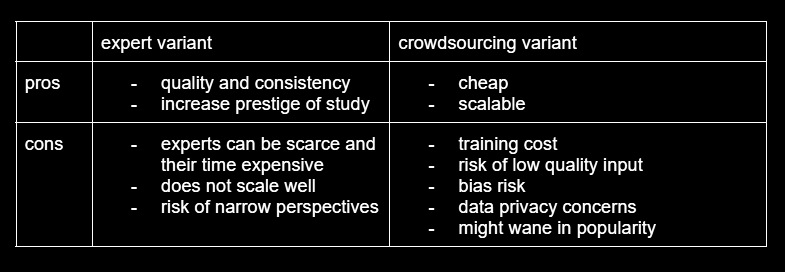
\includegraphics[width=0.5\textwidth]{./images/experts-vs-crowdsource.png}
    \caption{Differences between approaches}
    \label{fig:example}
\end{figure}


\section{Argdown}

The UBI topic could be represented like this in Argdown:

`[Statement 1]: Universal basic income should be implemented.
  + UBI can reduce poverty and inequality.
    + UBI can provide a safety net for individuals who are struggling to make ends meet, which can help reduce poverty and inequality.
    + UBI can reduce the bureaucratic costs associated with means-tested welfare programs, which can make it easier and more cost-effective to provide assistance to those in need.
    - UBI can create a disincentive for work, as individuals may choose not to work if they have a guaranteed basic income, which can actually increase poverty levels.
    - UBI can be expensive to implement and may require significant tax increases, which can be a burden on working individuals and families.
  + UBI can promote entrepreneurship and innovation.
    + UBI can provide a financial cushion that allows individuals to take risks and pursue entrepreneurial ventures without worrying about financial insecurity.
    + UBI can reduce income inequality, which can provide more opportunities for individuals from all socioeconomic backgrounds to start businesses and innovate.
    - UBI can decrease the incentive for individuals to work hard and innovate, as they may feel comfortable living off their basic income and not pursuing other opportunities.
    - UBI can increase taxes and government spending, which can stifle economic growth and discourage innovation.
  - UBI can lead to inflation and decrease the value of currency, causing more harm than good.
    + UBI can increase demand for goods and services, which can lead to price increases and inflation.
    + UBI can reduce the incentive to work and increase consumption, leading to an excess of money in the economy which can also contribute to inflation.
    - UBI can provide a more stable source of income for individuals, which can lead to less economic volatility and decrease the likelihood of inflation.
    - UBI can reduce the need for government welfare programs, which can lead to cost savings and help to mitigate inflationary pressures.
    - UBI can discourage people from working and contribute to a decline in productivity, which can have negative effects on the economy.
  - UBI can discourage people from working and contribute to a decline in productivity, which can have negative effects on the economy.
    + UBI can reduce the incentive for individuals to work, leading to a decrease in productivity and economic output.
    + UBI can create a disincentive for individuals to pursue higher education and acquire skills that can contribute to the economy.
    - UBI can provide a safety net for individuals who may have difficulty finding work or need to take time off to care for family members, which can actually increase productivity by reducing financial stress.
    - UBI can provide a more stable source of income, which can encourage individuals to pursue creative and entrepreneurial endeavors that can contribute to the economy.
    `

\section{AIFdb}

\chapter{Requirements and analysis}

\section{Stakeholder analysis}
The stakeholders can be listed as:

Users of the Lully application, including the various use cases:
- team leaders working to build compatible teams
- technical and fiction writers seeking to invent new arguments
- developers seeking to align artificial intelligences with a given set of values 
- open-minded individuals trying to better understand others' positions, for instance in a value conflict in a team

And the other categories:
- Developers of the application 
- Researchers - all users of the data produced by Lully
- Society at large, as the project can be expected to promote in effect mutual understanding and ethical decision-making, which can be expected to have wide scope positive impacts.

\section{Requirements}
To avoid the pitfalls of human annotation, a quantitative approach should be pursued. A diverse range of both source texts and human participants is needed. 

\subsection{Functional requirements}

Annotation takes two fundamental forms: the opinions on particular statements, and the judgement on the relations between any two given statements.
The former can  take a boolean form, as under classical logic, or more exotic ones, such as four valued logic, as outlined in  \cite{priest_many-valued_2008}
Having collection of such data points would allow to gauge global opinions on every statement in the database.

Judgement on the relations of two statment has been tried many times before, as is outlined above. That could be whether the relation is expressing agreement, disagreement, sarcasm, or an emotion.

Application should be able to import data from other formats, such as Argdown or AIFdb. That import could be user side, when a file conforming to either standard is uploaded, or on the backend as a admin tool where big chunks of data can be imported.
There is also the export angle, where arguments made in Lully can be safely exported into a file conforming to either standard. That would allow researchers that use the data downstream to more easily feed it into their processing pipelines.

A sample user flow can be imaged as the following:
- Player finds the landing page
- Browses the list of topics popular at the moment
- clicks to read more, is redirected to the app page
- there is presented with a tutorial how to engage with the systemn: read, and contribute.

Over the following week:
- user completes a small number of interactions with the application
- user integrates the app importing some content on their own, be it from Twitter or other dynamic corpora (for instance a blog article to annotate to understand it better)
- user continues to grow their use of the app, perhaps using it as a note taking app

Proof of concept stage:
- allow users to see and add new statements
- have a basic gamification feature with stats about the number of contributions and badges

If the project progresses beyond the proof-of-concept stage:
- allow users to flag inappropriate content
- provide administrative analytics 
- provide a way for information outflow for the researchers to access data

\subsubsection{Games}
\begin{itemize}
  \item Make ADUs game
  \item Swipe Game
  \item TruthGame 
  \item (pending) Syllogism based games
  \item (pending) Tree confirmation game
  \item (pending) combined game SwipeTruth
\end{itemize}
Swipe game is about deciding whether 2 statemnts are in support or attack relation to one another, or altogether not related.
TruthGame is about the user telling their opinion about a given statement. It is not the core feature compared to the relation one, but logically necessary.

SwipeTruth is a combination of the two games, SwipeGame and TruthGame, where the user first orients themselves with respect to a statement and then is presented with multiple statements that can either support it or reject it.
Make ADUs (Argumentative Discourse Units) is about performing the argument extraction from a given section.
Syllogism based games serve to uncover enthymemes as mentioned in (Razuvayevskaya and Teufel 2017). 
Tree confirmation is when user sees an argument and can confirm whether it makes sense as a whole. If not, the user can adjust relations between individual statements within the argument tree.

These games cover most of the 5 steps of argument mining. 
Argument extraction is not covered, or is covered implicitly when users submit sections from source texts. Argument segmentation is handled in the makeADUS game. Identification of relations and labeling is done through SwipeGame. The last step, argument completion is performed through the syllogism based games, and confirmed through the tree confirmation game.


Critical thinking skills as imcreasing user interest.

\subsection{Non-Functional requirements}
Performance: The system shall respond to user presses under half a second for most of the interactions.
Usability: The user interface shall be intuitive and easy to navigate
Security and data privacy: The system shall implement robust user authentication and access control measures to protect user data, prevent unauthorized access.
Compatibility: The system shall be compatible with a range of devices, including iOS and Android and web.
Maintainability: The codebase shall be well-documented with consistent coding standards to make it easy to maintain and update in the future.

\section{Stretch goals}
The goal of creating a full fledge application, an 'argument suite' so to speak, comparable to products like Microsoft Word or Miscrosoft Powerpoint, but for arguments is a collosal one.
Greatly outside of the scope of a BSc project, possibly requiring thousands of person-hours with more experience.
Given that, many of the features of the complete data collection system can be only outlined without implementation.
That type centers on the live multiplayer features. Two players would be able to adversarially create 2 branches of a root node, one for support and one in response, as mentioned in the literature reivew. 
This could be extended for the purpose of live streamed debates, with stakes. Such events have a niche following on platforms such as Twitch or Twitter Spaces.
Debate handled there could be reflected live in the tree. This would not necessarily require the speakers themselves would type - the moderators could fill that role.
Impact of the debate could be measured empirically by usingthe global statustics feature to guage the agreement status on a debate item before and after the debate
This could be narrowed to only the users who have been watching the debate as well.

\section{Success criteria}
The final criteria is the volume of quality annotated corpus. It could be uploaded to AIFdb. 
This will be known after performing quality control on the main argument database created through the lifetime of the app. 

The other criterion is the number of downloads - if larger than 150 it is \href{https://www.statista.com/statistics/1119893/average-number-downloads-united-states-app-publishers/}{ better than global average, if more than 1300, over global average}.


These data will be achieved from app publisher analytics.

\subsection{Ensuring data quality}
Data quality is a necessary property of the output dataset. Debate data of poor quality is readily available on the internet.

Potential approaches to ensuring data is of sufficient quality can be split into pre-collection and post-collection measures. Collection is the moment of addition of data into the database. These collection methods are summarized in Table \ref{tab:collection}.

  \begin{table}[h!]
      \centering
    \begin{tabular}{|l|p{4cm}|}
\toprule
Pre-collection measures:  & \begin{itemize}[left=0pt,topsep=0pt]\item only verified users being able to use the App
  \item automatic detection of invalid inputs (empty strings, etc)
  \item not sending the data created by the first time users to the database to prevent mistakes on the early stage of usage.
  \item putting users in adversarial scenarios where their performance is assessed by peers (social status as \href{https://dictionary.cambridge.org/dictionary/english/have-skin-in-the-game}{`skin in the game'})
\end{itemize} \\
\midrule

 Post-collection measures:  & \begin{itemize}[left=0pt,topsep=0pt]
  \item validation of each input by multiple validators.  
  \item rewarding user input on the basis of agreement with other users (adapting the Keynesian Beauty Contest \cite{keynes_general_1935})

\end{itemize} \\
\bottomrule
    \end{tabular}
    \caption{A summary of collection measures}

 \end{table}\label{tab:collection}

\newpage

\chapter{Design}
This section will be aboud...... top down view of organization and functional capabilities.
Design of the app is before all about the user journey. That process is outlined below. Based on that as a constraint, we can plan out the frontend and then a compatible backend.
Frontend is composed of 2 parts, 2 different capabilities - the games for data collection and the experience points system. The first is gamification on small timescale, the latter on long.

\section{User journey}
\begin{itemize}
  \item user discovers Lully through channels such as app stores or word of the mouth
  \item user downdloads tha app and makes a account
  \item user logs in
  \item user browses the available topics
  \item user click on topic they like
  \item user plays the SwipeGame for a couple of minutes in the context of that topic
  \item user adds more arguments
  \item user earns points and progresses on the ladder
  \item user can share game results and be active in the community
\end{itemize}

\section{Backend data structures related to the arguments}
By sectioning off the data structured related to the purpose, excluded are authentication structures such as passwords and gamification structures.
Backend is structured in terms of tables in a relational database with PostgresSQL:
\begin{itemize}
  \item authors
  \item sections
  \item source texts
  \item statements
  \item topics
  \item user relation
\end{itemize}
Authors table contains author's name and reference to their wikipedia page for reference. It is linked to the source texts table as each texts has 1 author. That table also links to some external page the text itself is available - be it a public domain text or a blogpost on author's page. source texts are referenced in turn in 'sections', which are short passages used as quotes by the users.
Each statement can reference a section so that its origin can be tracked. Statements contain a reference to the user who added them and to the section of the source text they belong to (if applicable), as well as data fields: text contents and number of views. Topics contain references to statements of a common theme.
user relation is the key element of the application. It is the table where users provide support/attack relations between a pair of statements. 
Supabase provides authentication mechanism inbuilt into the backend.

Data can be imported from AIFdb. The exact data structure is not preserved in the current version of Lully, as AIFdb uses text coordinate system and a complex syntax. Making Lully align with it would be effort-heavy yet does not add much to the core functionality. Lossy data import must be good enough for the current purposes.

\section{Backend gamification representation}

It is structured into these PostgresSQL tables:
- achievements
- gamer profiles 
- top gamers 
Achievements is a simple table listing possible achievements each user may have. They are referenced to the gamer_profiles in a linker table. Gamer profiles recounts the number of user's contributions as experience points.
Top gamers is a PostgresSQL View, that is a custom query, which in this case returns a leaderboard of all players, sorted by number of experience points.

\section{Frontend interactions with the backend}

Frontend is an \href{https://expo.dev/}{Expo} React Native application that uses supabase-js library to interact with the backend.
Contents of the tables about source texts (with their authors) and topics are received on the frontend when the user previews source texts or topics. On clicking a given source texts, snippets (sections) from it are displayed.
Notable packages include Tailwindcss for styling, Typescript for types and Jest for testing. 

\section{Data inputs - Game Modes}
\subsection{Multiplayer features}
\begin{itemize}
  \item Daily challenge mode
  \item Seasonal modes
  \item Debate game
  \item (pending) Vote for investigation
\end{itemize}
Daily challenge mode would be a time limited competition, encouraging daily use and driving up ALP (Average Lifetime Play). It would confer a 'streak' status for a player who performs some minimum set of tasks, for instance a set of 5 different ones. That should not take long time, preferably under 5 minutes.

Seasonal modes could be statements or topics algorithmically suggested to players more during certain times of the year. Many busqinesses do such events as an accepted practice.

Debate mode would be a type of game where two players aim to prove / disprove a given statement, the root node of an otherwise empty argument tree.  A snapshot of the global support for a statement is gauged at the start of a debate, then two players each add new statement nodes to the argument. Each addition of a node to the argument tree would constitute a move.
A node can be added to any node in the tree that the opponent put, or the root node. Otherwise a new support node can be added to an existing move.

Another distinction between game-states comes from  \cite{rienks_argument_2005}. That is the observations that there are more types of issues than just 'yes/no' issues. They call them: A/B issues, yes-no issue, open issue. It is obvious that the yes-no issue might be the simplest to implement, yet it would be a lost opportunity to forsake the other modes.
Such issues are defined as Investigations, with many possible Statements being the candidate solutions to them. After a certain time elapses the Investigation is closed. As a community event this can be expected to be quite engaging.

\section{Gamification design}

\section{User Resources}
\begin{itemize}
  \item experience points 
  \item competition - leaderboard feature, in different game modes
  \item achievements - badges for completing certain milestones, for each game mode
\end{itemize}

User can access their account panel and see their achievements as well as experience points. These are not public. The leaderboard is public though, and a user's place can be seen, alongside the list of top 10 players. On the backend a trigger happens whenever a user makes an action so that their experience points are updated.
\section{User satisfaction}
For optimization of user satisfaction a tagging system is added to the topics and the source text tables, which points at various \href{https://adancewithbooks.wordpress.com/2019/09/22/a-small-list-of-trigger-warnings-you-can-use/}{trigger warnings}.
\newpage

\chapter{Implementation and testing}
Platform choice - there is a possibility of a web appplication or a mobile one.

The proof of concept also highlighted some of the challenges of working with Supabase and React Native, particularly in terms of data transmission and validation, cross-update of topics, and update algorithms for the data structure and gamification part.

In this chapter, I will discuss the implementation and testing of the application. The goal of the implementation phase was to build a functional and user-friendly application that fulfilled the design outlined in the previous chapter.

\section{Software choice}

\subsection{Frontend}
The choice of the platoform is the first concern. The best way is to address many of them - that is a website and mobile format. Choosing only one would drive away some users. 
There is a limited but developed choice in software solutions that allow developers to deliver multi-platform software. They all offer roughly similar levels of user experience, performance, crossplatforms, customizabiltiy. Likewise, accessibility and community support are all attested for these libraries.
Therefore other considerations can come into play, taking into account the constraints of the projects. Frameworks with easier onboarding experience and more automation are easier to fit in given the limited time. Easy onboarding experience means good documentation and familiar syntax.
Author is the most familiar with the Javascript / Typescript language and React as the state management system.

FLutter is a popular multi-platform framework from Google, yet it is written in Dart. Learning a new language would be a bottleneck on the whole project.
https://en.wikipedia.org/wiki/Flutter_(software)

NativeScript is another frontend mobile framework, enjoyed by many developers. It can be combined with Angular or Vue for state management.
https://en.wikipedia.org/wiki/NativeScript
Given author's skills presented above, that is less than optimal. Yet there is another framework that does not have this disadvantage.

Expo SDK is a multiplatform library and SDK that uses Typescript and ReactNative.
Moreover it provids deployment options as part of the SDK. That is the feature that lead to choice of expo as the frontend framework of choice. 
https://expo.dev/

\subsection{Backend}

Bakcend needs to be able to maange the data, and integrate well with the frontend, implying a well-maintained javascript client library.
Moreover, the usual desiderata for software choice in this domain apply, which are: scalablity, security, reliablity, cost-effectiveness, degree of technical support, flexibility. 

comparison of SDKs
https://github.com/firebase/firebase-js-sdk
https://github.com/supabase/supabase-js
https://github.com/pocketbase/js-sdk
https://github.com/aws-amplify/amplify-js

Platforms that have these features are many, most notably AWS Amplify and Firebase. WHat is problematic about these two is that they are closed source and force vendor lock-in. 
That is inflexible. There is a number of open source alternatives, most prominently Supabase and Pocketbase. The advantage of the latter is that is a more mature project. What is more, a free tier hosting is offered, offering an escape from the complexities of self-hosting. 

https://pocketbase.io/faq

AWS Amplify
https://aws.amazon.com/amplify/


\section{Architecture}

\section{Frontend screenshots and snippets}
% todo add the example here

\section{Backend screenshots and snippets}
% todo add the example here

\section{challenges}
% todo outline this more, delete from code traps
- reading AIFdb and the 80 characters 
- choosing the backend data representation
- readign in files from remote to use many possible text sources for arguments
- not using supabase types from the start, but doing a frontend only prototype. that created more work for later.

\section{Code traps}
One of the main challenges faced during the implementation was dealing with code traps, which slowed down the development process. Another important aspect was the design of the interface and screens in the application in a logical way to ensure a smooth user experience. Data transmission and validation cross-update of topics were also significant considerations to ensure the reliability of the application.

Furthermore, I had to develop update algorithms for both the data structure and gamification bit. These allowed the users to track their progress using their place on the contributor leaderboard. To achieve this, I had to ensure that the algorithms were efficient and effective in updating user data, and that the progress bars reflected user progress accurately.

I also integrated AIFdb to translate the data from the AIF database to the application, which was a lossy translation.

Finally, I worked with the Argdown library, which proved to be a challenging but powerful tool for structuring and visualizing arguments. Despite the challenges of working with this library, it provided significant benefits in helping us to structure and present complex arguments in a user-friendly way.

In summary, the implementation phase of the project involved a range of challenges and considerations, from designing an intuitive user interface to developing update algorithms for gamification elements. I also had to work with a variety of tools and libraries, including AIFdb and Argdown. 

Ultimately, I was unable to achieve the goals and create a functional and user-friendly application that has the potential to help users better understand complex arguments. The lessons learned from this phase will be valuable for potential future development efforts focused on adding new functionalities.

\newpage

\chapter{Results and discussion}

The proof of concept version of the  project yielded cautiously optimistic results. While I was not able to conduct a wider experimental study due to time and ethics constraints, the findings from the limited sample size suggest that Lully is effective in achieving project objectives. 

User feedback was the last part of the project. I recognize the importance of creating a smooth user flow and ensuring that the order of screens is logical and intuitive. Beyond limited the testing on humans, multiplayer features are one aspect of the application that was considered in the beginning yet failed to materialize due to time constraints. 

\section{Methodology}
The problem was approached through prototype development. Prototypes of new games were presented in varying intervals. The stack of React Native plus Supabase was not decided from the start, only from December on. It was a partly new stack for me, which caused a learning curve and led to many of the lessons listed below.

Having created a frontend with Expo React Native February saw effforts toward backend integration. Read access was a success, while write access required adjustment of permissions. AIFdb integration was tried in parallel, as has Argdown been. These two venues have been largely unfruitful, as the communities behind these projects aren't quite alive anymore. The only data extractable from there is the statements themselves, but which are often in very niche topics. That causes limited applicability to the Lully project. 

\subsection{Lessons learned in design}
Theere is a number of pitfalls I ran into concerning both the frontend and the backend of the application. The main issue in the frontend of the application was the layout of the screens. It needs to be logical for the user and allow for a maintainable and clear keeping of state between the screens for the developer experience. Querying supabase, that is the backend, is not as straightforward as one might imagine in edge cases with many join tables. Supabase uses PostgresSQL as the relational database and interacting with it, writing SQL queries was not easy. 

Overall the authentication flow was less plug-and-play than expected and required some tweaking. 

Argdown implementation is one of the biggest failures of the project. The repository is not developed fully and not updated regularily. The API is not complete, that is not all of the operations thatn can be done through text interface can be done with Argdown. Another effort to create a complete interfacing library would be necessary.

\section{Further directions}
Several next steps for this project can be outlined. The first objective is to expand the scope of the proof of concept to make it accessible to a larger user base. This may involve actions such as improving the user interface smoothness and clarity, optimizing performance, adding multiplayer features.

The multiplayer mode would give the users an ability to engage in debates with each other. It is hoped it would foster productive dialogue and build empathy across divides.
Users will be challenged on their assumptions in an organic way, hopefully leading to constructive conversations. Multiplayer mode would promote a nuanced understanding of complex issues.

Not only human debaters could be available on Lully. Training an AI agent could result in a brilliant and entertaining conversation partner. Technically that could be approached through using a pretrained model and fine-tuning it on Lully data.

Having validated the proof of concept, it is seen that there is value in the expanding the reach and improving capabilities of Lully. It can become a compelling tool that will benefit users across many topics and create datasets more research can be based on.

\newpage

\chapter{Conclusions}

The Lully project is a proof of concept for mobile app crowdsourcing tool designed to create argument datasets while improving the critical thinking skills of the users. 

The proof of concept is on a mobile application that allows users to explore different topics, from philosophical problems and dilemmas, to policy questions for small towns. Users can evaluate the ethical and epistemic implications of their preferences and see how much other people agree with them. The app uses the Games With A Purpose paradigm to motivate the players. Gamification elements in Lully are constituted by a linear experience system and complimentary granular achievement system. This combination aims to encourage users to engage with the content and explore different games inside Lully. It is worth noting that 'gamification' is primarily a user retention measure and more classical marketing approaches would be necessary for user acquisition.

The proof of concept was designed and implemented using Supabase, a cloud database service, and React Native, a mobile application development framework. React Native was used with Expo library, an open source configuration suite that allows developers to code once and deploy to both mobile and web. I faced some challenges working with these technologies, as it took some time to work out edge cases and get intuition for how some aspects work.

The Lully project team learned several important lessons during the implementation and testing of the proof of concept. They gained experience in working with Supabase and React Native, and learned about the importance of a smooth user flow and logical order of screens. They also gained insights into the challenges of using the Argdown library and working with the AI-Framework Database (AIFDB) for data translation.

Overall, the Lully project proof of concept represents an important step towards the development of crowdsourced tools for dataset generation critical thinking. While there are still challenges to be addressed, the results of the proof of concept demonstrate the potential of the approach.

\newpage

\printbibliography

\end{document}
